\documentclass[
    parskip=half, 
    twoside=false,
    twocolumn=true,
    fontsize=11pt,
]{scrarticle}
\usepackage{xcolor}
\definecolor{seeblau}{HTML}{00A9E0}
\definecolor{seegrau}{HTML}{9AA0A7}

\definecolor{seeblau1}{HTML}{CCEEF9}
\definecolor{seeblau2}{HTML}{A6E1F4}
\definecolor{seeblau3}{HTML}{59C7EB}
\definecolor{seeblau4}{HTML}{00A9E0}
\definecolor{seeblau5}{HTML}{008ECE}


\usepackage{graphicx}
\usepackage{amsmath}
\usepackage{subcaption}
\usepackage{wrapfig}
\usepackage[english]{babel}
\usepackage{blindtext}
\usepackage{microtype}
\usepackage{siunitx}
\usepackage[utf8]{inputenc}
\usepackage{csquotes}
\usepackage{nicefrac}
\usepackage[T1]{fontenc}
\usepackage{amsfonts}
\usepackage{amssymb}
\usepackage{tikz}

\usepackage{siunitx}

\usepackage{libertinus, libertinust1math}
\usepackage{roboto}

\setkomafont{disposition}{\normalfont\sffamily}


% not recommended with KOMA-script
% make table of contents sans-serif
% \usepackage{tocloft}
% \renewcommand\cftchappagefont{\normalfont}
% \renewcommand\cftchapfont{\normalfont}
% \renewcommand\cftchappresnum{\bfseries}
% \renewcommand\cftchapaftersnum{}
% \renewcommand{\cftchapfont}{\sffamily}
% \renewcommand{\cftsecfont}{\sffamily}
% \renewcommand{\cftsubsecfont}{\sffamily}
% \renewcommand{\cftchappagefont}{\sffamily}
% \renewcommand{\cftsecpagefont}{\sffamily}
% \renewcommand{\cftsubsecpagefont}{\sffamily}

% caption
\usepackage{caption}
\captionsetup{
	% font={sf},
	labelfont={sf, bf, color=seeblau},
	labelsep=quad,
	labelformat=simple,
}

% links
\usepackage{hyperref}
\hypersetup{
	colorlinks=true,
	linkcolor=seeblau,
	citecolor=seeblau,
	urlcolor=seeblau,
	% hidelinks=true
}

% bibliography
\usepackage[
	style=numeric-comp, % comp = compressed 4,5,6,7 -> 4-7
	sorting=none,		% Sort by appearance
	% autocite = superscript,
	% backref=true,
	hyperref=true,
	url=true,
	maxbibnames=100
]{biblatex}
\DefineBibliographyStrings{english}{%
    backrefpage  = {see p.}, % for single page number
    backrefpages = {see pp.} % for multiple page numbers
}

% remove issue
\AtEveryBibitem{%
  \clearfield{number}
}

\usepackage{float}
% \floatplacement{figure}{h}
% \floatplacement{table}{H}

% loosen float placement rules
\renewcommand{\topfraction}{0.8}
\renewcommand{\bottomfraction}{.8}
\renewcommand{\textfraction}{0.1}
\renewcommand{\floatpagefraction}{.9}
% make floats less likely to be placed on a separate page
\setcounter{totalnumber}{9}
\setcounter{topnumber}{9}
\setcounter{bottomnumber}{9}

% decrease space between floats and text
\setlength{\textfloatsep}{0.5cm}
\setlength{\floatsep}{0.5cm}


\usepackage{adjustbox}

\usepackage{datetime}
\newdateformat{dotdate}{
	\twodigit{\THEDAY}.\twodigit{\THEMONTH}.\THEYEAR
}
\newdateformat{monthyeardate}{%
  \monthname[\THEMONTH] \THEYEAR}


% header and footer
\usepackage[
  markcase=noupper
]{scrlayer-scrpage}% activates pagestyle scrheadings automatically
\clearpairofpagestyles
\setkomafont{pageheadfoot}{\normalfont\sffamily}
\setkomafont{pagenumber}{\normalfont\sffamily}
% \chead*{\color{seegrau} Draft \dotdate\today}
\ofoot*{\pagemark}
\ohead*{\rightmark}


\usepackage{ifthen}
\newcommand{\markieren}[4]{
    \ifthenelse{\equal{#1}{}}{}{\adjustbox{padding=3pt, bgcolor=seeblau1, margin=-1pt}{\strut{\sffamily\robotoMedium{#1}}}\\}
    \ifthenelse{\equal{#2}{}}{}{\adjustbox{padding=3pt, bgcolor=seeblau2, margin=-1pt}{\strut{\sffamily\robotoMedium{#2}}}\\}
	\ifthenelse{\equal{#3}{}}{}{\adjustbox{padding=3pt, bgcolor=seeblau3, margin=-1pt}{\strut{\sffamily\robotoMedium{#3}}}\\}
	\ifthenelse{\equal{#4}{}}{}{\adjustbox{padding=3pt, bgcolor=seeblau4, margin=-1pt}{\strut{\sffamily\robotoMedium{#4}}}}
}


\begin{document}

\title{title}
\subtitle{subtitle}
\author{Aurel Müller-Schoenau, Leon Oleschko}
\date{\dotdate\today}


% make a custom title page
\begin{titlepage}
    \sffamily
    \vspace*{3cm}
    {
        \fontsize{32}{32}
        \markieren{}{}{Evanescent light scattering}{Optical Tweezers}
    }
    \vspace{.25cm}\\
    {
        \Large
        Aurel Müller-Schoenau, Leon Oleschko\\
        Supervised by Aasdf Kasdf
        \vspace{.05cm}\\
        13.11.2024
        \vspace{.25cm}\\
        \normalsize
        Physikalisches Fortgeschrittenenpraktikum 2\\
        Universität Konstanz
    }
    \vfill
    {
        \normalfont\normalsize
        Abstract auf Englisch (10-15 Zeilen)
        \blindtext[2]
    }
    \vfill
    \begin{flushright}
        Available at \url{www.github.com/leoole100/fp2}.
    \end{flushright}
\end{titlepage}

\section{Introduction}

\subsection{Physical Principles}
kompakten Zusammenstellung der physikalischen Grundlagen

Mean square deviation and velocity autocorrelation:
\url{https://de.wikipedia.org/wiki/Mittlere_quadratische_Verschiebung#Verbindung_zur_Geschwindigkeitsautokorrelation}
\begin{align}
    &&\left<v(t)\cdot v(t+\tau)\right> &= - \frac{d}{d\tau} \frac{\left<r^2(\tau)\right>}{6\tau}\\
    \Rightarrow&&\left<r^2(\tau)\right> &= 6 \int_0^\tau (\tau - s) \left<v(0) \cdot v(s)\right> ds
\end{align}

The maxwell boltzmann relations (from script) are given by
\begin{align}
    P(x) &\propto \exp\left(- \frac{V(x)}{k_B T}\right)\\
    V(x) &\propto - \frac{\log{P(x)}}{k_B T}
\end{align}


\section{Methods}
Mit einer Skizze des Versuchsaufbaus

\section{Procedure}

\pagebreak
\section{Results}

All recorded data and the analysis is available at \url{www.github.com/leoole100/fp2}.

\subsection{Transmission Light Microscopy}
\begin{figure*}[h]
    \centering
    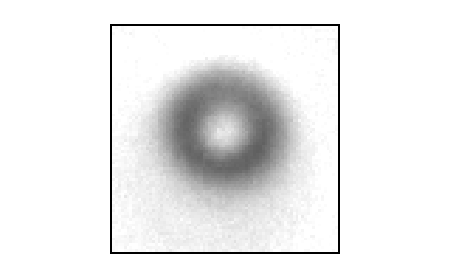
\includegraphics{figures/01_01_1_particle.pdf}
    \caption{Transmission light microscopy of a single particle, after normalization.}
\end{figure*}

\begin{figure*}[h]
    \centering
    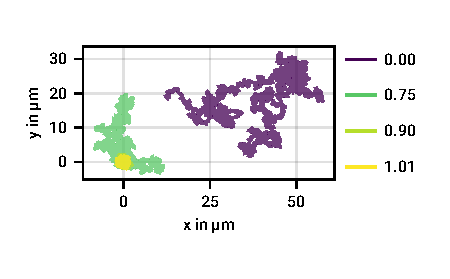
\includegraphics{figures/01_02_1_trajectories.pdf}
    \caption{Tracked trajectories relative to trap center.}
\end{figure*}

\begin{figure*}[h]
    \centering
    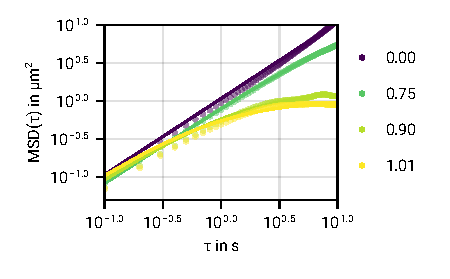
\includegraphics{figures/01_02_2_msd.pdf}
    \caption{Mean Square Displacement}
\end{figure*}

\begin{figure*}[h]
    \centering
    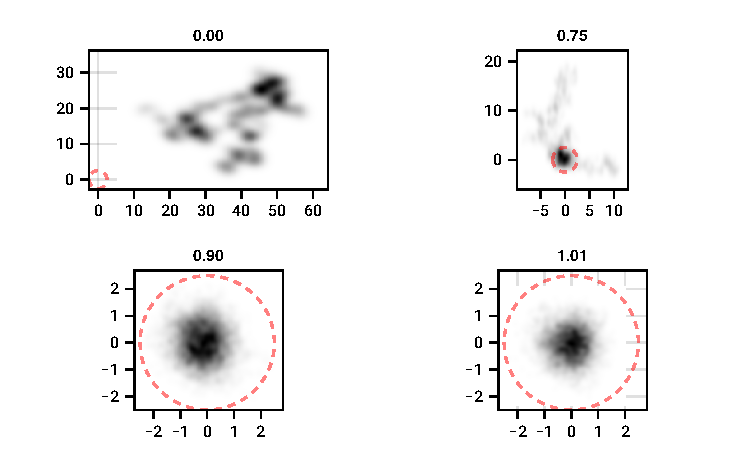
\includegraphics{figures/01_03_1_bivariate.pdf}
    \caption{Bivariate histogram for different trap strengths, relative to mean position, different scale in um.}
\end{figure*}

\begin{figure*}
    \centering
    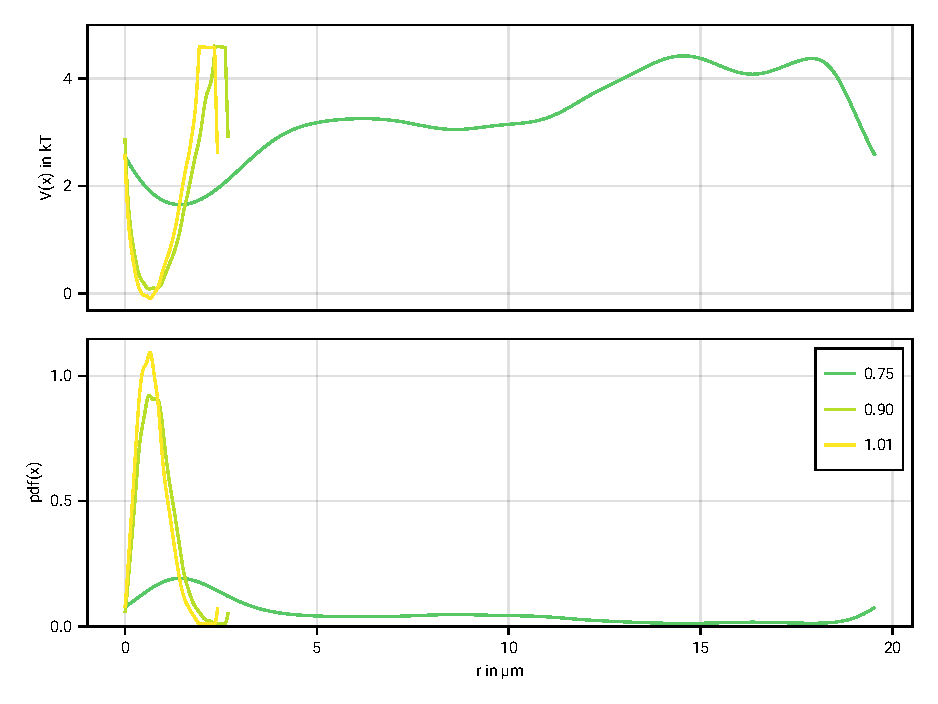
\includegraphics{figures/01_03_2_radial.pdf}
    \caption{Distance to center of trap. Qualitatively, the same if center is mean per track or "real" center.}
\end{figure*}

\begin{figure*}
    \centering
    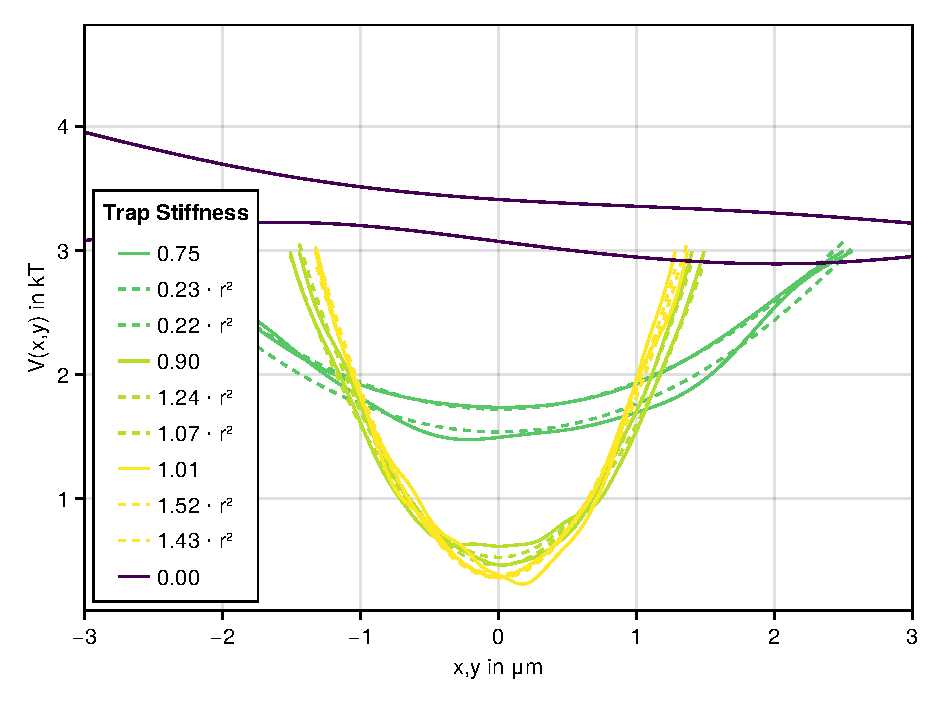
\includegraphics{figures/01_03_3_axis.pdf}
    \caption{Grouped by axis, relative to mean.}
\end{figure*}

\begin{figure*}
    \centering
    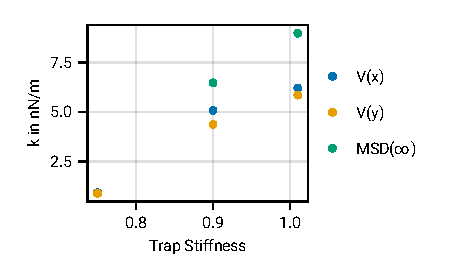
\includegraphics{figures/01_03_4_spring_constants.pdf}
    \caption{Differently measured spring constants.}
\end{figure*}

\pagebreak
\section{Discussion}


\end{document}